\documentclass[9pt,twocolumn,twoside]{gsajnl}
\newcommand{\sme}[1]{\textcolor{red}{\bf #1}}
\newcommand{\yang}[1]{\textcolor{orange}{\emph{\scriptsize  #1}} }
\graphicspath{{Figure_Table/}} \newcommand{\beginsupplement}{        \setcounter{table}{0}
        \renewcommand{\thetable}{S\arabic{table}}        \setcounter{figure}{0}
        \renewcommand{\thefigure}{S\arabic{figure}}     }

\articletype{inv} 
\newcommand{\X}{\textcolor{red}{\bf X\,}} \newcommand{\citex}{\textcolor{red}{\bf (CITE)\,}} 
\newcommand{\jri}[1]{\textcolor{red}{ \emph{ #1}} }  \title{Deleterious genetic loads and their contributions to heterosis in genomic selection}  \author[$\ast$, 1]{Jinliang Yang} \author[$\ast$, 1, 2]{Sofiane Mezmouk} \author[$\dagger$]{Andy Baumgarten}
\author[$\ddagger$]{Rita H. Mumm}
\author[$\ast$, $\S$, 3]{Jeffrey Ross-Ibarra} 
\affil[$\ast$]{Department of Plant Sciences, University of California, Davis, CA 95616, USA}
\affil[$\S$]{Center for Population Biology and Genome Center, University of California, Davis, CA 95616, USA}
\affil[$\dagger$]{DuPont Pioneer, Johnston, IA 50131, USA}
\affil[$\ddagger$]{Department of Crop Sciences, University of Illinois at Urbana-Champaign, Urbana, IL 61801, USA}

\keywords{heterosis; deleterious; genomic selection; diallel; GERP; maize} 
\runningtitle{Genomic Selection Using GERP score} 
\correspondingauthor{Jeffrey Ross-Ibarra}

\begin{abstract}
Complementation of the deleterious alleles carried by the inbred parents may contribute to the vigorous performance, or heterosis, of the hybrid progenies. The detection of deleterious alleles was previous limited to the protein-coding regions. With the genomic evolutionary rate profiling (GERP), we extended the definition of deleterious alleles to the genome-wide. In total, about 86 million base-pairs, which make up 4.2\% of the maize genome, were detected as evolutionary conserved sequences in both genic and non-genic regions. Here we take advantage of evolutionary measures of sequence conservation to ask whether sites with prior evidence of functionality can inform genomic selection (GS) models. We tested this idea using a partial diallel cross of 12 maize inbred lines. We sequenced the genomes of the parents and phenotyped both parents and hybrids for seven phenotypic traits across one environment in three years. We made use of an identity-by-decent analysis of the parents to identify haplotype blocks, and scored blocks in hybrids using a weighted sum of the GERP conservation score. We find that incorporating sequence conservation improves prediction accuracies in a five-fold cross-validation experiment for several traits \emph{per se} as well as heterosis for those traits. Because most variation at conserved sites is deleterious, we interpret these results as consistent with the simple complementation model for heterosis. Overall, this work demonstrates the importance of incorporating evolutionary information in GS and its potential usage in plant breeding.  \end{abstract}

\setboolean{displaycopyright}{true}
\RequirePackage[normalem]{ulem} \RequirePackage{color}\definecolor{RED}{rgb}{1,0,0}\definecolor{BLUE}{rgb}{0,0,1} \providecommand{\DIFadd}[1]{{\protect\color{blue}\uwave{#1}}} \providecommand{\DIFdel}[1]{{\protect\color{red}\sout{#1}}}                      \providecommand{\DIFaddbegin}{} \providecommand{\DIFaddend}{} \providecommand{\DIFdelbegin}{} \providecommand{\DIFdelend}{} \providecommand{\DIFaddFL}[1]{\DIFadd{#1}} \providecommand{\DIFdelFL}[1]{\DIFdel{#1}} \providecommand{\DIFaddbeginFL}{} \providecommand{\DIFaddendFL}{} \providecommand{\DIFdelbeginFL}{} \providecommand{\DIFdelendFL}{} 
\begin{document}

\maketitle
\thispagestyle{firststyle}
\marginmark
\firstpagefootnote
\correspondingauthoraffiliation{Department of Plant Sciences, University of California, Davis, CA 95616, USA. Email: rossibarra@ucdavis.edu}
\blfootnote{\textsuperscript{2}These authors contributed equally to this work}
\blfootnote{\textsuperscript{3}Current address: KWS SAAT AG, Grimsehlstr. 31, 37555 Einbeck, Germany}
\vspace{-11pt}






\lettrine[lines=2]{\color{color2}T}{}he phenomenon of heterosis \DIFaddbegin \DIFadd{or hybrid vigor }\DIFaddend has been observed \DIFdelbegin \DIFdel{for many speciesacross species}\DIFdelend \DIFaddbegin \DIFadd{across many species}\DIFaddend , from yeast \citep{Shapira2014} to \DIFaddbegin \DIFadd{plants \mbox{\citex{}
}and }\DIFaddend vertebrates \citep{Gama2013}. 
\DIFdelbegin \DIFdel{Recent studies indicated that the complementation of the }\DIFdelend \DIFaddbegin \DIFadd{A number of hypotheses have been put forth to explain the phenomenon, including gene dosage \citex, }\X \DIFadd{\citex, and }\X \DIFadd{\citex. 
Complementation of recessive }\DIFaddend deleterious alleles, \DIFdelbegin \DIFdel{which fit the classical dominance genetic model, may play an important role in determining heterosis \mbox{\citep{Charlesworth2009}
}. }\DIFdelend \DIFaddbegin \DIFadd{however, remains the simplest genetic explanation \mbox{\citep{Charlesworth2009}
}, and is supported by considerable empirical evidence \citex.
}

\DIFaddend Deleterious alleles were arisen from new mutations during meiosis. In maize, about 90 new mutations were generated per meiosis \citep{Clark2005}, majority of which were deleterious according to empirical estimates \citep{Joseph2004}. In a natural outcross population, the negative effects on fitness of these deleterious alleles make them subject to be selection against\DIFdelbegin \DIFdel{. Therefore, deleterious alleles were }\DIFdelend \DIFaddbegin \DIFadd{, which lead the deleterious alleles to be }\DIFaddend maintained in a low frequency \citep{Eyre-Walker2007}. \DIFaddbegin \DIFadd{But the deleterious alleles could not be completerly purged. 
}\DIFaddend 

In maize, the total number of mildly deleterious mutations is substantial because of the exponential growth of population size after domestication. The modern breeding probably aims to remove these deleterious mutations and pyramiding beneficial alleles for agronomical \DIFdelbegin \DIFdel{important traits}\DIFdelend \DIFaddbegin \DIFadd{purposes}\DIFaddend . In practice, the relatively homogeneous maize germplasm pool was artificially divided into different heterotic groups \citep{Heerwaarden2012}. It enabled the improvement of germplasm pools to be conducted in a parallel fashion, and therefore, facilitated the breeding efficiency. Using this hybrid breeding approach, the maize yield has been steadily improved since the early 20th century \citep{duvick2001biotechnology}. However, removing deleterious mutations in low recombination regions or in tightly linked regions become less effective. Studies indicated that residual heterozygosity correlates negatively with recombination \citep{Gore2009, McMullen2009} and the low recombination is effective over long period of time \citep{Haddrill2007}. As a consequence, the deleterious alleles would be accumulated in the low recombination regions, such as the pericentromeric regions in maize, and the vigorous performance could be realized by combining two sets of non-deleterious or beneficial alleles in repulsion state, thus lead to pesudo-overdominance. A recent QTL study identified loci controlling for heterosis are enriched in centromeric regions \citep{Lariepe2012}, which partly support this pesudo-overdominance hypothesis.

Despite the importance of deleterious alleles in contributing to heterosis, they have not been systematically investigated probably because of their low frequencies in the population and \DIFdelbegin \DIFdel{minor effects individually}\DIFdelend \DIFaddbegin \DIFadd{mostly exhibiting minor effects}\DIFaddend . Here, we employed a genomic selection (GS) approach to simultaneously estimate genome-wide deleterious variants in a half diallel population. The diallel population \DIFaddbegin \DIFadd{was }\DIFaddend composed of a set of hybrids\DIFaddbegin \DIFadd{, which }\DIFaddend enabled us to explore different modes of inheritance of the deleterious variants. And the study can be conducted with millions of variants but using relative little sequencing efforts. In \DIFdelbegin \DIFdel{a }\DIFdelend \DIFaddbegin \DIFadd{our }\DIFaddend previous study, \DIFdelbegin \DIFdel{we found the enrichment of deleterious SNPs }\DIFdelend \DIFaddbegin \DIFadd{deleterious SNPs were found to be enriched }\DIFaddend in a SNP set identified by GWAS \citep{Mezmouk2014}. The deleterious variants in the study were defined as non-synonymous mutations in the coding regions. Clearly, deleterious variants are not limited to coding regions. Here, we expanded the characterization of deleterious variants to genome-wide \DIFdelbegin \DIFdel{by }\DIFdelend using genomic evolutionary rate profiling (GERP) \citep{Cooper2005}. By incorporating \DIFdelbegin \DIFdel{the }\DIFdelend GERP information in \DIFdelbegin \DIFdel{the GS model}\DIFdelend \DIFaddbegin \DIFadd{GS models}\DIFaddend , we demonstrated the prediction accuracies were significantly improved not only for some traits \emph{per se}, but \DIFaddbegin \DIFadd{aslo }\DIFaddend for some heterosis transformations \DIFaddbegin \DIFadd{(especially for traits exhibiting high levels of hereosis)}\DIFaddend . Further studies indicated that \DIFdelbegin \DIFdel{the genetic architectures varied among traits with different levels of heterosis; and the prediction accuracies with different }\DIFdelend \DIFaddbegin \DIFadd{joint effects of deleterious alleles with additive and dominant }\DIFaddend modes of inheritance \DIFdelbegin \DIFdel{would perform differently}\DIFdelend \DIFaddbegin \DIFadd{may contribute to heterosis}\DIFaddend .


\section*{Materials and Methods} 
\DIFdelbegin \DIFdelend 

\subsection*{Plant \DIFdelbegin \DIFdel{Material }\DIFdelend \DIFaddbegin \DIFadd{material }\DIFaddend and \DIFdelbegin \DIFdel{Phenotypic Data}\DIFdelend \DIFaddbegin \DIFadd{phenotypic data}\DIFaddend }
\DIFdelbegin \DIFdel{Twelve }\DIFdelend \DIFaddbegin \DIFadd{We selected 12 }\DIFaddend maize inbred lines\DIFdelbegin \DIFdel{were selected and crossed in a half diallel fashion without considering reciprocal effects }\DIFdel{. 
The experimental design includes the }\DIFdelend \DIFaddbegin \DIFadd{, broadly representative of corn belt maize germplasm \mbox{\citep{mikel2006evolution}
}, as parents of a partial diallel population. 
Each parent in a cross was used as both male and female and the resulting seed was bulked. 
We evaluated the }\DIFaddend 66 F1 hybrids, \DIFdelbegin \DIFdel{the }\DIFdelend 12 inbred parents \DIFdelbegin \DIFdel{, and 2 }\DIFdelend \DIFaddbegin \DIFadd{and two }\DIFaddend current commercial check hybrids \DIFdelbegin \DIFdel{grown in }\DIFdelend \DIFaddbegin \DIFadd{in the field in Urbana, IL over three years (2009-2011) in }\DIFaddend an incomplete block design with \DIFdelbegin \DIFdel{3 replications; hybrids and inbreds were grouped separately.  
The test was grown at Urbana, IL in 2009, 2010, and 2011.  }\DIFdelend \DIFaddbegin \DIFadd{three replicates each year.  
}\DIFaddend Plots consisted of \DIFdelbegin \DIFdel{4 }\DIFdelend \DIFaddbegin \DIFadd{four }\DIFaddend rows, with all observations taken from the inside \DIFdelbegin \DIFdel{2 }\DIFdelend \DIFaddbegin \DIFadd{two }\DIFaddend rows to minimize effects of shading and maturity differences from adjacent plots.  
\DIFdelbegin \DIFdel{Both inbred lines and the 66 resulting hybrids were field evaluated. Phenotypic data was collected for }\DIFdelend \DIFaddbegin \DIFadd{We measured }\DIFaddend plant height (PHT, in cm), ear height (EHT, in cm), days to 50\% silking (DTS), days to 50\% pollen shed (DTP), anthesis-silking interval (ASI, in days), grain yield adjusted to 15.5\% moisture (adj GY, in bu/A), and test weight (\DIFdelbegin \DIFdel{TWT}\DIFdelend \DIFaddbegin \DIFadd{TW}\DIFaddend , in pounds)\DIFdelbegin \DIFdel{. 
}\DIFdelend \DIFaddbegin \DIFadd{. 
Overall mean phenotypic values for each cross can be found at \citex.
}\DIFaddend 

\DIFaddbegin \DIFadd{We estimated }\DIFaddend Best Linear Unbiased \DIFdelbegin \DIFdel{Estimation (BLUE}\DIFdelend \DIFaddbegin \DIFadd{Estimates (BLUEs}\DIFaddend ) of the genetic effects \DIFdelbegin \DIFdel{were calculated with }\DIFdelend \DIFaddbegin \DIFadd{in }\DIFaddend ASReml-R \DIFdelbegin \DIFdel{following the }\DIFdelend \DIFaddbegin \DIFadd{\mbox{\citep{gilmour2009asreml}
}with the following }\DIFaddend linear model: 
\[\DIFdelbegin \DIFdel{y}\DIFdelend \DIFaddbegin \DIFadd{Y}\DIFaddend _{ijkl} = \mu + \varsigma_{i} + \delta_{ij} + \beta_{jk} + \alpha_{l} +  \varsigma_{i} \cdot \alpha_{l} + \varepsilon\]
where 
\DIFdelbegin \DIFdel{$y_{ijkl}$ }\DIFdelend \DIFaddbegin \DIFadd{$Y_{ijkl}$ }\DIFaddend is the phenotypic value of the $l^{th}$ genotype evaluated in the $k^{th}$ block of the $j^{th}$ replicate within the $i^{th}$ \DIFdelbegin \DIFdel{environment}\DIFdelend \DIFaddbegin \DIFadd{year}\DIFaddend ; 
$\mu$, the overall mean; 
$\varsigma_{i}$, the fixed effect of the $i^{th}$ \DIFdelbegin \DIFdel{environment}\DIFdelend \DIFaddbegin \DIFadd{year}\DIFaddend ;
$\delta_{ij}$, the fixed effect of the $j^{th}$ replicate nested in the $i^{th}$ \DIFdelbegin \DIFdel{environment}\DIFdelend \DIFaddbegin \DIFadd{year}\DIFaddend ; 
$\beta_{jk}$, the random effect of the $k^{th}$ block nested in the $j^{th}$ \DIFdelbegin \DIFdel{block}\DIFdelend \DIFaddbegin \DIFadd{replicate}\DIFaddend ; 
$\alpha_{l}$, the the fixed genetic effect  of the $l^{th}$ individual; 
$\varsigma_{i} \cdot \alpha_{l}$, the interaction effect of the $l^{th}$ individual with the $i^{th}$ \DIFdelbegin \DIFdel{environment}\DIFdelend \DIFaddbegin \DIFadd{year}\DIFaddend ; 
$\varepsilon$, the model residuals. 

\DIFdelbegin \DIFdel{Heterosis for each hybrid was then estimated by both best- and mid-parent heterosis ($BPH$ and $MPH$, respectively) }\DIFdelend \DIFaddbegin \DIFadd{We estimated best-parent heterosis (BPH) as}\DIFaddend :
\DIFdelbegin \[\DIFdel{ MPH_{ij}=\hat{G_{ij}}-\frac{1}{2}(\hat{G_{i}}+\hat{G_{j}}) }\]
\DIFdelend \[ BPH_{min,ij}=\hat{G_{ij}}-min(\hat{G_{i}} ,\hat{G_{j}}) \] 
\[ BPH_{max,ij}=\hat{G_{ij}}-max(\hat{G_{i}} ,\hat{G_{j}}) \]
where $\hat{G_{ij}}$, $\hat{G_{i}}$ and $\hat{G_{j}}$ are the genetic values of the hybrid and its two parents $i$ and $j$. $BPH_{min}$ was used instead of $BPH_{max}$ for days to anthesis. \DIFdelbegin \DIFdelend \DIFaddbegin \jri{what about ear height and DTS?}
\DIFaddend 

\subsection*{Sequencing \DIFdelbegin \DIFdel{of Founder Lines }\DIFdelend and \DIFdelbegin \DIFdel{SNP Callings}\DIFdelend \DIFaddbegin \DIFadd{Genotyping}\DIFaddend }

\DIFaddbegin \DIFadd{We extracted }\DIFaddend DNA from the \DIFdelbegin \DIFdel{twelve inbred lines was CTAB extracted \mbox{\citep{Doyle1987}
}and Covaris sheared for Illumina }\DIFdelend \DIFaddbegin \DIFadd{12 inbred lines following \mbox{\citet{Doyle1987}
}and sheared the DNA on a Covaris (Woburn, Massachusetts) for }\DIFaddend library preparation. \DIFdelbegin \DIFdel{The DNA libraries }\DIFdelend \DIFaddbegin \jri{do we need details on library prep? at least a citation?}
\DIFadd{Libraries }\DIFaddend were then sequenced \DIFdelbegin \DIFdel{to an average coverage of 10X }\DIFdelend \DIFaddbegin \jri{where? what length reads? insert size?}\DIFaddend . 

\DIFdelbegin \DIFdel{Raw paired reads (reverse and forward for each sequence), were trimmed for }\DIFdelend \DIFaddbegin \DIFadd{We trimmed  raw sequence reads for }\DIFaddend adapter contamination with Scythe  \DIFdelbegin \DIFdel{package }\DIFdelend (\url{https://github.com/vsbuffalo/scythe}) \DIFdelbegin \DIFdel{which calculate the probability of having a contamination given the adapter sequence, the number of mismatches and sequence quality. The reads were then trimmed }\DIFdelend \DIFaddbegin \DIFadd{and }\DIFaddend for quality and sequence length ($\geq 20$ nucleotides) with Sickle \DIFdelbegin \DIFdel{package }\DIFdelend (\url{https://github.com/najoshi/sickle}). 
\DIFdelbegin 
\DIFdel{Read pairs, kept after filtering,  were mapped }\DIFdelend \DIFaddbegin \DIFadd{We mapped filtered reads }\DIFaddend to the maize B73 reference genome (AGPv2) with bwa-mem \citep{Li2009B}\DIFdelbegin \DIFdel{. Reads, }\DIFdelend \DIFaddbegin \DIFadd{, keeping reads }\DIFaddend with mapping quality (MAPQ) higher than 10 and with a best alignment score higher than the second best one \DIFdelbegin \DIFdel{, were kept }\DIFdelend for further analyses.
\DIFdelbegin 
\DIFdelend \DIFdelbegin \DIFdel{Single }\DIFdelend \DIFaddbegin \DIFadd{We called single }\DIFaddend nucleotide polymorphisms (SNPs) \DIFdelbegin \DIFdel{were called with mpileup }\DIFdelend \DIFaddbegin \DIFadd{using the $mpileup$ function }\DIFaddend from samtools utilities \citep{Li2009}. 
To deal with \DIFdelbegin \DIFdel{paralogy, which is a major problem in maize sequence mapping \mbox{\citep{Chia2012}
}, all }\DIFdelend \DIFaddbegin \DIFadd{known issues with paralogy in maize \mbox{\citep{Chia2012}
}, }\DIFaddend SNPs were filtered to \DIFdelbegin \DIFdel{a) }\DIFdelend be heterozygote in less than 3 inbred lines, \DIFdelbegin \DIFdel{b) }\DIFdelend have a mean minor allele depth \DIFdelbegin \DIFdel{over all genomes }\DIFdelend of at least 4, \DIFdelbegin \DIFdel{c) }\DIFdelend have a mean depth over all individuals lower than 30 and \DIFdelbegin \DIFdel{d) }\DIFdelend have missing/heterozygote alleles in \DIFdelbegin \DIFdel{less }\DIFdelend \DIFaddbegin \DIFadd{fewer }\DIFaddend than 6 inbred lines\DIFdelbegin \DIFdel{(allelic information for at least 15 hybrids in the partial diallel design)}\DIFdelend . 

\DIFdelbegin \subsection*{\DIFdel{Haplotype identification and SNP annotation}}

\DIFdelend \DIFdelbegin \DIFdel{All missing alleles were then imputed with BEAGLE package \mbox{\citep{Browning2009}
}and }\DIFdelend \DIFaddbegin \DIFadd{We used the fastIBD method implemented in BEAGLE \mbox{\citep{Browning2009,Browning2011}
}to impute missing data and identify regions of }\DIFaddend identity by descent \DIFdelbegin \DIFdel{regions }\DIFdelend (IBD) between the 12 inbred lines\DIFdelbegin \DIFdel{were identified with BEAGLE's fastIBD method \mbox{\citep{Browning2011}
}. The pairwise IBD region starts and ends were used to delimit haplotipic blocs where several inbred lines shared a homogenous haplotypes.}\DIFdelend \DIFaddbegin \DIFadd{. We then defined haplotype blocks as contiguous regions within which there were no IBD break points across all pairwise comparisons of the parental lines (Figure \ref{fig:defineibd}). 
}\DIFaddend 

\DIFdelbegin \DIFdel{The SNPs were annotated as synonymous and non-synonymous with the software polydNdS from the analysis package of libsequence  \mbox{\citep{Thornton2003}
}using the first transcript of each gene in B73 5b filtered gene set. 
Deleterious effects of amino acid changes were then predicted with both SIFT \mbox{\citep{Ng2003, Ng2006}
}and MAPP \mbox{\citep{Stone2005}
}software packages as described by \mbox{\citep{Mezmouk2014}
}.
}\DIFdelend 
\DIFdelbegin \DIFdel{Genomic evolutionary rate profiling (GERP) }\DIFdel{, which estimates the evolutionary constraint by quantifying substitution deficits after multiple genome alignments, was obtained from }\DIFdel{for AGPv2. 
}\DIFdelend 
\DIFdelbegin \subsection*{\DIFdel{Association mapping}}
\DIFdel{SNP association with heterosis (BPH and MPH) was tested assuming dominance/recessivity of the reference allele or assuming overdominance where only the heterozygote alleles are expected to be significant. For each SNP, root mean square error were used to select the best fitting model. 
Haplotype association with heterosis were tested comparing the heterozygote alleles to all homozygote ones all confounded. 
}\DIFdelend \DIFaddbegin \subsection*{\DIFadd{Genomic selection using IBD blocks incorporated with GERP scores}}
\DIFaddend 

\DIFdelbegin \subsection*{\DIFdel{Genomic-enabled prediction with GERP score}}

\DIFdel{A haplotype based genomic selection (GS) strategy was conceived by using the IBD blocks as the explanatory variables containing conservation information. The reference genome sites with GERP score />0 were considered as conserved sites and genomic variations at these sites were deemed as deleterious. To incoporate the conservation information into IBD blocks, SNPsfalling into a given IBD block were added up using their GERP scores as the conservation estimates of the IBD block}\DIFdelend \DIFaddbegin \DIFadd{We used genome-wide estimates of evolutionary constraint \mbox{\citep[GERP][]{Davydov2010}
}estimated by \mbox{\citet{rodgers2015recombination}
}. 
Haplotype blocks were weighted by the summed GERP scores of all deleterious (GERP score $>0$) SNPs}\DIFaddend . 
This estimation was calculated \DIFdelbegin \DIFdel{using a python script gerpIBD (}\DIFdel{)with additive and dominant models. 
Under the additive model, 2 x GERP score was assigned to the homozygous loci with }\DIFdelend \DIFaddbegin \DIFadd{under both additive and dominant modes of inheritance using a custom python script available at (}\url{https://github.com/yangjl/zmSNPtools}\DIFadd{). 
For a particular SNP with a GERP score $g$, the }\DIFaddend non-reference \DIFdelbegin \DIFdel{SNP calls; 1 x GERP score was assigned to the heterozygous loci; and 0 was assigned to the homozygous loci with reference SNP calls. }\DIFdelend \DIFaddbegin \DIFadd{homozygote was assigned a value of $2g$, the heterozygote a value of $g$, and the reference homozygote a value of 0.  
}\DIFaddend Under the dominant model, \DIFdelbegin \DIFdel{1 x GERP score was assigned to both the homzygous loci with }\DIFdelend \DIFaddbegin \DIFadd{both the heterozygote and the }\DIFaddend non-reference \DIFdelbegin \DIFdel{SNP calls and heterozygous loci; 0 was assigned to homozygous loci with reference SNP calls.
}
\DIFdel{seven phenotypic traits were trained with the conservation statistics in IBD block as genotype.
A Bayesian-based approach, BayesC }\DIFdel{, was employed for the GS experiments. To conduct predict, }\DIFdelend \DIFaddbegin \DIFadd{homozygote were assigned a value of $g$, with }\DIFaddend the \DIFaddbegin \DIFadd{reference homozygote again assigned a value of 0.
To conduct prediction, a 5-fold cross-validation method was used, dividing the }\DIFaddend diallel population  \DIFdelbegin \DIFdel{was randomly  divided into training }\DIFdelend \DIFaddbegin \DIFadd{randomly  into training (80\%) }\DIFaddend and validation sets \DIFdelbegin \DIFdel{for }\DIFdelend \DIFaddbegin \DIFadd{(20\%)  }\DIFaddend 10 times\DIFdelbegin \DIFdel{according to a 5-fold cross-validation method. 
First, the BayesC model was trained independently on each of the trainingset. Second, the prediction accuracy was }\DIFdelend \DIFaddbegin \DIFadd{. 
The BayesC option from GenSel4 \mbox{\citep{habier2011extension}
}was used for model training, using 41,000 iterations and removing the first 1,000 as burn-in. }\jri{this said chains but I think you mean iterations?}
\DIFadd{After model training, prediction accuracies were }\DIFaddend obtained by comparing the predicted \DIFdelbegin \DIFdel{and observed phenotypes on the conresponding validation set. 
}
\DIFdel{In addition, the }\DIFdelend \DIFaddbegin \DIFadd{breeding values with the observed phenotypes in the corresponding validation sets. 
For comparison, }\DIFaddend GERP scores were circularly shuffled \DIFdelbegin \DIFdel{. The cross-validation }\DIFdelend \DIFaddbegin \DIFadd{by 50k SNPs windows ($> 100$Mb) 10 times to estimate a null conservation score for each IBD blocks. 
Cross-validation }\DIFaddend experiments using the circularly shuffled data were conducted on the same training and validation sets.  


\DIFdelbegin \subsection*{\DIFdel{Data Access}}
\DIFdelend 


\DIFdelbegin \textit{\DIFdel{GENETICS}} \DIFdel{is committed to the open access to all primary data (see }\DIFdel{). Please indicate where data can be found (supplemental files, public repository, or published with another paper).
}
\DIFdelend \section*{Results}


\subsection*{Genetic values, heritability and heterosis\DIFdelbegin \DIFdel{transformations of a half diallel population}\DIFdelend }

A \DIFdelbegin \DIFdel{half }\DIFdelend \DIFaddbegin \DIFadd{partial }\DIFaddend diallel population was created using 12 maize inbred lines (Figure \ref{fig:pvp-pheno}a). 
Two of them are important public inbreds, B73 and Mo17. And the other ten of \DIFdelbegin \DIFdel{them are }\DIFdelend proprietary inbreds (LH1, LH123HT, LH82, PH207, 4676A, PHG39, PHG47, PHG84, PHJ40, PHZ51) that have expired from Plant Variety Protection (PVP) and represent \DIFaddbegin \DIFadd{much of }\DIFaddend the lineage of key heterotic germplasm pools used in present-day commercial corn hybrids. 
\DIFdelbegin \DIFdel{The set is diverse enough to facilitate a broad sweep of the heterotic sub-groups that comprise U.S. commercial germplasm. }\DIFdelend From this population, phenotypic data were collected for seven traits of interest during 2009-2011\DIFdelbegin \DIFdel{. The phenotypic traits are }\DIFdelend \DIFaddbegin \DIFadd{: }\DIFaddend anthesis-silking interval (ASI, in days), days to 50\% pollen shed (DTP), days to 50\% silking (DTS), ear height (EHT, in cm), grain yield adjusted to 15.5\% moisture (GY, in bu/A), plant height (PHT, in cm), and test weight (TW, in pounds).

\DIFdelbegin \DIFdel{The best }\DIFdelend \DIFaddbegin \DIFadd{Best }\DIFaddend linear unbiased estimators (BLUEs) for genotypes of the seven traits were derived from mixed linear models (Table S1). 
In the models, all fixed effects were significant (Wald test \emph{P} value \DIFdelbegin \DIFdel{< 0.05}\DIFdelend \DIFaddbegin \DIFadd{$<0.05$}\DIFaddend ) for all traits except ASI\DIFaddbegin \DIFadd{, }\DIFaddend for which the effect of \DIFdelbegin \DIFdel{the }\DIFdelend replicates within environments were not significant. 
As shown in \DIFdelbegin \DIFdel{the }\DIFdelend Figure \ref{fig:pvp-pheno}b, \DIFdelbegin \DIFdel{the }\DIFdelend BLUE values were normally distributed (normality test \emph{P} values \DIFdelbegin \DIFdel{> 0.05). 
The broad sense heritability of the }\DIFdelend \DIFaddbegin \DIFadd{$>0.05$). 
Broad sense heritability for these }\DIFaddend traits ranged from 0.65 for ASI to 0.95 for PHT. 
\DIFdelbegin \DIFdel{With }\DIFdelend \DIFaddbegin \DIFadd{Using }\DIFaddend the parental phenotypic data, we \DIFdelbegin \DIFdel{conducted heterosis transformations using better-parental heterosis }\DIFdelend \DIFaddbegin \DIFadd{then estimated best-parent heterosis }\DIFaddend (BPH) \DIFdelbegin \DIFdel{and percent better-parental heterosis (pBPH)}\DIFdelend \DIFaddbegin \DIFadd{for each trait}\DIFaddend .  
Because the selected inbred lines are \DIFdelbegin \DIFdel{commercial }\DIFdelend \DIFaddbegin \DIFadd{commercially }\DIFaddend relevant and fairly elite in performance, hybrids in this population exhibit \DIFdelbegin \DIFdel{relative }\DIFdelend \DIFaddbegin \DIFadd{relatively }\DIFaddend low hybrid vigor (overall mean \DIFdelbegin \DIFdel{pBPH }\DIFdelend \DIFaddbegin \DIFadd{percent BPH }\DIFaddend = 0.3\% $\pm$ 0.4\%) \DIFdelbegin \DIFdel{compared to their parents for most of the }\DIFdelend \DIFaddbegin \DIFadd{for most }\DIFaddend traits except GY (mean \DIFdelbegin \DIFdel{pBPH }\DIFdelend \DIFaddbegin \DIFadd{percent BPH }\DIFaddend = 95\% $\pm$ 16\%, Figure \ref{fig:pBPH}). 
Finally, general and specific combining ability (GCA \DIFdelbegin \DIFdel{ans }\DIFdelend \DIFaddbegin \DIFadd{and }\DIFaddend SCA) were estimated following \citep{Falconer1996}. 
\DIFdelbegin \DIFdel{The }\DIFdelend GCA and SCA varied \DIFdelbegin \DIFdel{according to the }\DIFdelend \DIFaddbegin \DIFadd{among }\DIFaddend traits (Table S2) \DIFdelbegin \DIFdel{. For the GY, }\DIFdelend \DIFaddbegin \jri{please add ref to actual table}\DIFadd{, but }\DIFaddend B73, PHG47 and PHG39 \DIFdelbegin \DIFdel{are the top three inbred lines that combining better with others}\DIFdelend \DIFaddbegin \DIFadd{showed the greatest GCA }\jri{or should this say SCA?} \DIFadd{for grain yield}\DIFaddend .

\subsection*{Evolutionary constraint information for genomic variants}

\DIFdelbegin \DIFdel{In this study, all }\DIFdelend \DIFaddbegin \DIFadd{All }\DIFaddend twelve inbreds were sequenced to an average depth of $\sim$10X\DIFdelbegin \DIFdel{. Reads were mapped to the maize B73 reference genome (AGPv2) with bwa-mem. After filtering of depth, heterozygosity and missingness, }\DIFdelend \DIFaddbegin \DIFadd{, resulting in a filtered set of }\DIFaddend 13.8 million SNPs\DIFdelbegin \DIFdel{were kept for further analysis, including 1.9 million SNPs in genic regions and 361,280 in protein coding regions}\DIFdelend . 
We estimated the allelic error rate \DIFdelbegin \DIFdel{by first comparing our genotype calls to those of }\DIFdelend \DIFaddbegin \DIFadd{using three independent data sets: for all individuals using }\DIFaddend 41,292 overlapping SNPs on the maize SNP50 bead chip \citep{Heerwaarden2012}; \DIFdelbegin \DIFdel{we then compared our SNP alleles for B73 and Mo17 with the 10,426,715 SNP previously identified in HapMap2 \mbox{\citep{Chia2012}
}; finally, we compared our SNPs to }\DIFdelend \DIFaddbegin \DIFadd{for all individuals using }\DIFaddend 180,313 overlapping SNPs identified through genotyping by sequencing (GBS) \citep{Romay2013}\DIFdelbegin \DIFdel{. The comparisons showed 99.12\% allele similarity with shared SNPs previously identified.  
}\DIFdelend \DIFaddbegin \DIFadd{; and for B73 and Mo17 using the 10,426,715 SNP from the HapMap2 project \mbox{\citep{Chia2012}
}. }\jri{add a sentence or two describing the error rates!}
\DIFaddend 

\DIFdelbegin \DIFdel{Evolutionary constraint information of GERP was obtained from \mbox{\citep{rodgers2015recombination}
}, which was computed by using rejected substitution rate relative to the neutral rate after multiple genome squences alignment \mbox{\citep{Davydov2010}
}. This approach could estimate the conservation information at the base-pair level,extending the definition of deleterious variants to non-genic regions compared to previous approaches of SIFT \mbox{\citep{ng2003sift}
}or MAPP \mbox{\citep{stone2005physicochemical}
}. In AGPv2, more }\DIFdelend \DIFaddbegin \DIFadd{More }\DIFaddend than 86 million \DIFdelbegin \DIFdel{bases ($\sim$4.2\% }\DIFdelend \DIFaddbegin \DIFadd{bp }\DIFaddend of the genome \DIFdelbegin \DIFdel{) were detected as evolutionary constraint bases with GERP score >0. From genome-wide of view, genomic sequences are evolutionarily constraint near the telomeric regions and the mean GERP scores dropped, in general, toward centromeric regions (Figure \ref{fig:dis1m}) with some exceptions at long arm of chromosome 1 and 4.  
}
\DIFdel{Although genomic sites with GERP score >0 showed evidence of under evolutionary constraint, they are not immune to mutate.
Indeed, in our diallel population, }\DIFdelend \DIFaddbegin \DIFadd{were annotated as conserved, with GERP scores $>0$ (Figure \ref{fig:gerpmaf}A and \ref{fig:dis1m}).
Nonetheless, }\DIFaddend 506,898 \DIFdelbegin \DIFdel{SNP variants were detected at sites where the GERP scores are bigger than zero (Figure \ref{fig:gerpmaf}A).
Consistent with previous study \mbox{\citep{rodgers2015recombination}
}, the minor allele frequencies (MAFs) of these SNPs were }\DIFdelend \DIFaddbegin \DIFadd{of these sites were found to segregate among the 12 inbred parents of our diallel.
The minor allele frequency of SNPs at conserved sites was }\DIFaddend negatively correlated with \DIFdelbegin \DIFdel{their GERP scores (Pearson's correlation test }\DIFdelend \DIFaddbegin \DIFadd{GERP score (Figure \ref{fig:gerpmaf}B; }\DIFaddend \emph{P} value < 0.05, \emph{r} = \DIFdelbegin \DIFdel{$-$0.08), indicating that the putative deleterious alleles tend to be purged and maintained in a low frequency in the population}\DIFdelend \DIFaddbegin \DIFadd{$-0.8$), consistent with the idea that variants at sites with more positive GERP scores are more deleterious and more strongly impacted by purifying selection}\DIFaddend .

\begin{figure}[htbp]
\centering
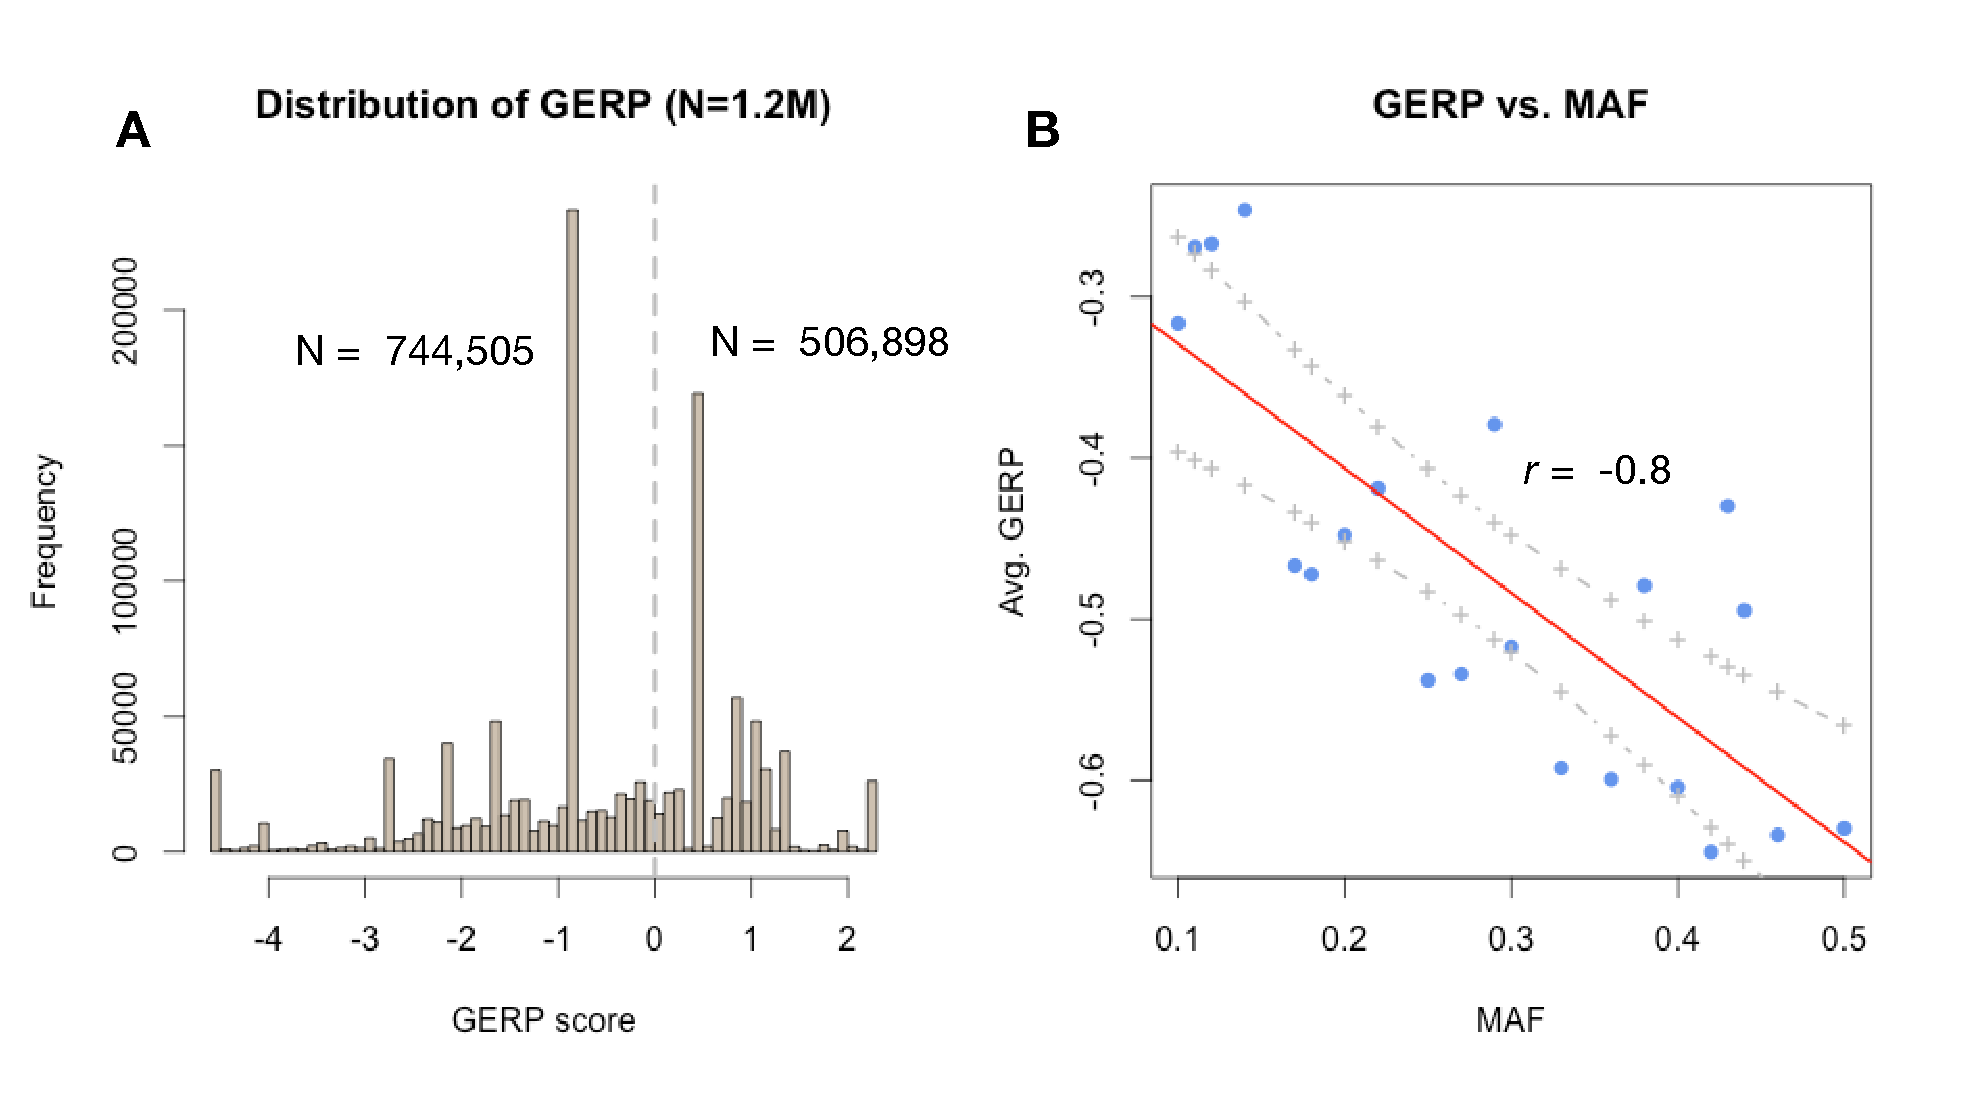
\includegraphics[width=\linewidth]{Figure_gerpmaf.pdf}
\caption{Distribution of GERP scores and relationship between GERP scores and MAFs. \textbf{(A)} GERP scores \DIFdelbeginFL \DIFdelFL{were }\DIFdelendFL extracted \DIFdelbeginFL \DIFdelFL{for }\DIFdelendFL \DIFaddbeginFL \DIFaddFL{from }\DIFaddendFL $\sim$1.2 million SNPs \DIFdelbeginFL \DIFdelFL{($\sim$10\% }\DIFdelendFL of the \DIFdelbeginFL \DIFdelFL{total SNPs) of the }\DIFdelendFL diallel population. \DIFdelbeginFL \DIFdelFL{The spikes in the histogram were because only limited genomes (N < 10? }\DIFdelFL{) were used in GERP calculation. }\DIFdelendFL \DIFaddbeginFL \jri{1.2M is just the sites where GERP scores were available, correct?} \DIFaddendFL \textbf{(B)} Mean GERP scores were calculated for each bin (bin size = 0.01) of minor allele frequency (MAF). The red  \DIFdelbeginFL \DIFdelFL{line }\DIFdelendFL and grey lines define the regression and its 95\% confidence interval.}
\label{fig:gerpmaf}
\end{figure}


\subsection*{Incorporatipn of GERP information improved prediction accuracies}

Genomic variants \DIFdelbegin \DIFdel{occured }\DIFdelend \DIFaddbegin \DIFadd{occurred }\DIFaddend at the evolutionary constraint sites were potentially deleterious. The phenotypic effects of these genetic loads and their contributions to heterosis become \DIFdelbegin \DIFdel{interesting}\DIFdelend \DIFaddbegin \DIFadd{an interesting area to explore}\DIFaddend . However, the population size in this study is relative small and SNPs detected at \DIFdelbegin \DIFdel{high GERP sites }\DIFdelend \DIFaddbegin \DIFadd{sites containing high GERP scores }\DIFaddend are generally in low \DIFdelbegin \DIFdel{frequcies. To alliviate }\DIFdelend \DIFaddbegin \DIFadd{frequencies. The statistical power to detect the separate effects of these putative deleterious alleles becomes very low. To alleviate }\DIFaddend the statistical limitations, we conceived a haplotype-based approach for \DIFdelbegin \DIFdel{genomic selection (GS)}\DIFdelend \DIFaddbegin \DIFadd{GS, which could add up individual effects of deleterious alleles in IBD blocks and estimate these IBD blocks simultaneously}\DIFaddend . To conduct the analysis, first of all, 55,000 IBD blocks were identified, which had an average size of 44,980 bp (ranged from 36 to 10,320,000 bp). IBD blocks having > 1-kb in size and containing \DIFdelbegin \DIFdel{at least one }\DIFdelend \DIFaddbegin \DIFadd{> 1 }\DIFaddend deleterious alleles (SNPs at sites with GERP scores >0) were kept for further analysis. Secondly, the GERP scores of SNPs in an IBD block were summed under both additive and dominant models. Those summed GERP scores on IBD blocks were considered as the measurements of the \DIFdelbegin \DIFdel{conserveness }\DIFdelend \DIFaddbegin \DIFadd{conservation }\DIFaddend of the haplotypes. More details of this procedure were illustrated in Figure \ref{fig:gerpibd}.      

A Bayesian-based statistical method (BayesC) \citep{habier2011extension} was employed for model training. Using a 5-fold cross-validation approach, the prediction accuracies of the real data and cicularly shuffled data were compared. As shown in Figure \ref{fig:gerpall}, for traits \emph{per se}, prediction accuracies were significantly (FDR < 0.05) improved for ASI and PHT when incorporating GERP information in the IBD blocks under the additive model; prediction accuracy was significantly improved for ASI under the dominant model. For heterosis transformation traits (BPH\DIFdelbegin \DIFdel{and pBPH}\DIFdelend ), incorporation of GERP scores improved BPH of GY under the additive model and improved BPH of DTP, DTS and TW under the dominant model \DIFdelbegin \DIFdel{; and the method improved predictions for pBPH of TW under the additive model and pBPH of GY under the dominant model }\DIFdelend (Figure \ref{fig:gerpall} \DIFdelbegin \DIFdel{C-F}\DIFdelend \DIFaddbegin \DIFadd{C and D}\DIFaddend , Supplementary table 3). In general, the average prediction accuracis were higher using the additive model (mean \emph{r} = 0.81 \DIFdelbegin \DIFdel{, 0.49 and 0.29 }\DIFdelend \DIFaddbegin \DIFadd{and 0.49 }\DIFaddend for traits \emph{per se} \DIFdelbegin \DIFdel{, BPH and pBPH}\DIFdelend \DIFaddbegin \DIFadd{and BPH}\DIFaddend ) than the dominant model (mean \emph{r} = 0.70 \DIFdelbegin \DIFdel{, 0.42 and 0.24}\DIFdelend \DIFaddbegin \DIFadd{and 0.42}\DIFaddend ). And the prediction accuracies decreased for predicting heterosis transformations (BPH\DIFdelbegin \DIFdel{and pBPH}\DIFdelend ) as compared to the predictions for traits \emph{per se}.

It was argued that SNPs in genic regions might have higher GERP scores than those in non-genic regions. The circular shuffling permutations may shift the high GERP scores to non-genic regions. If that is the case, the approach tended to weigh more on genic SNPs. To rule out this possibility, we elected SNPs with GERP scores >0 in genic regions only and did the circular shuffling to assign GERP scores to the same set of the selected SNPs. By doing this, the method will not take advantage of genomic positional information any more. Noted that in this study less number of SNPs was selected (N = 316, 983). Nevertheless, model prediction accuracies were significantly improved for traits \emph{per se} of GY under the additive model. For heterosis transformations, prediction accuracies were significantly improved for BPH of GY and PHT under the additive model and the prediction accuracy was significantly improved for pBPH of GY (Figure \ref{fig:genicsnp} and Table S4).   


\begin{figure}[htbp]
\centering
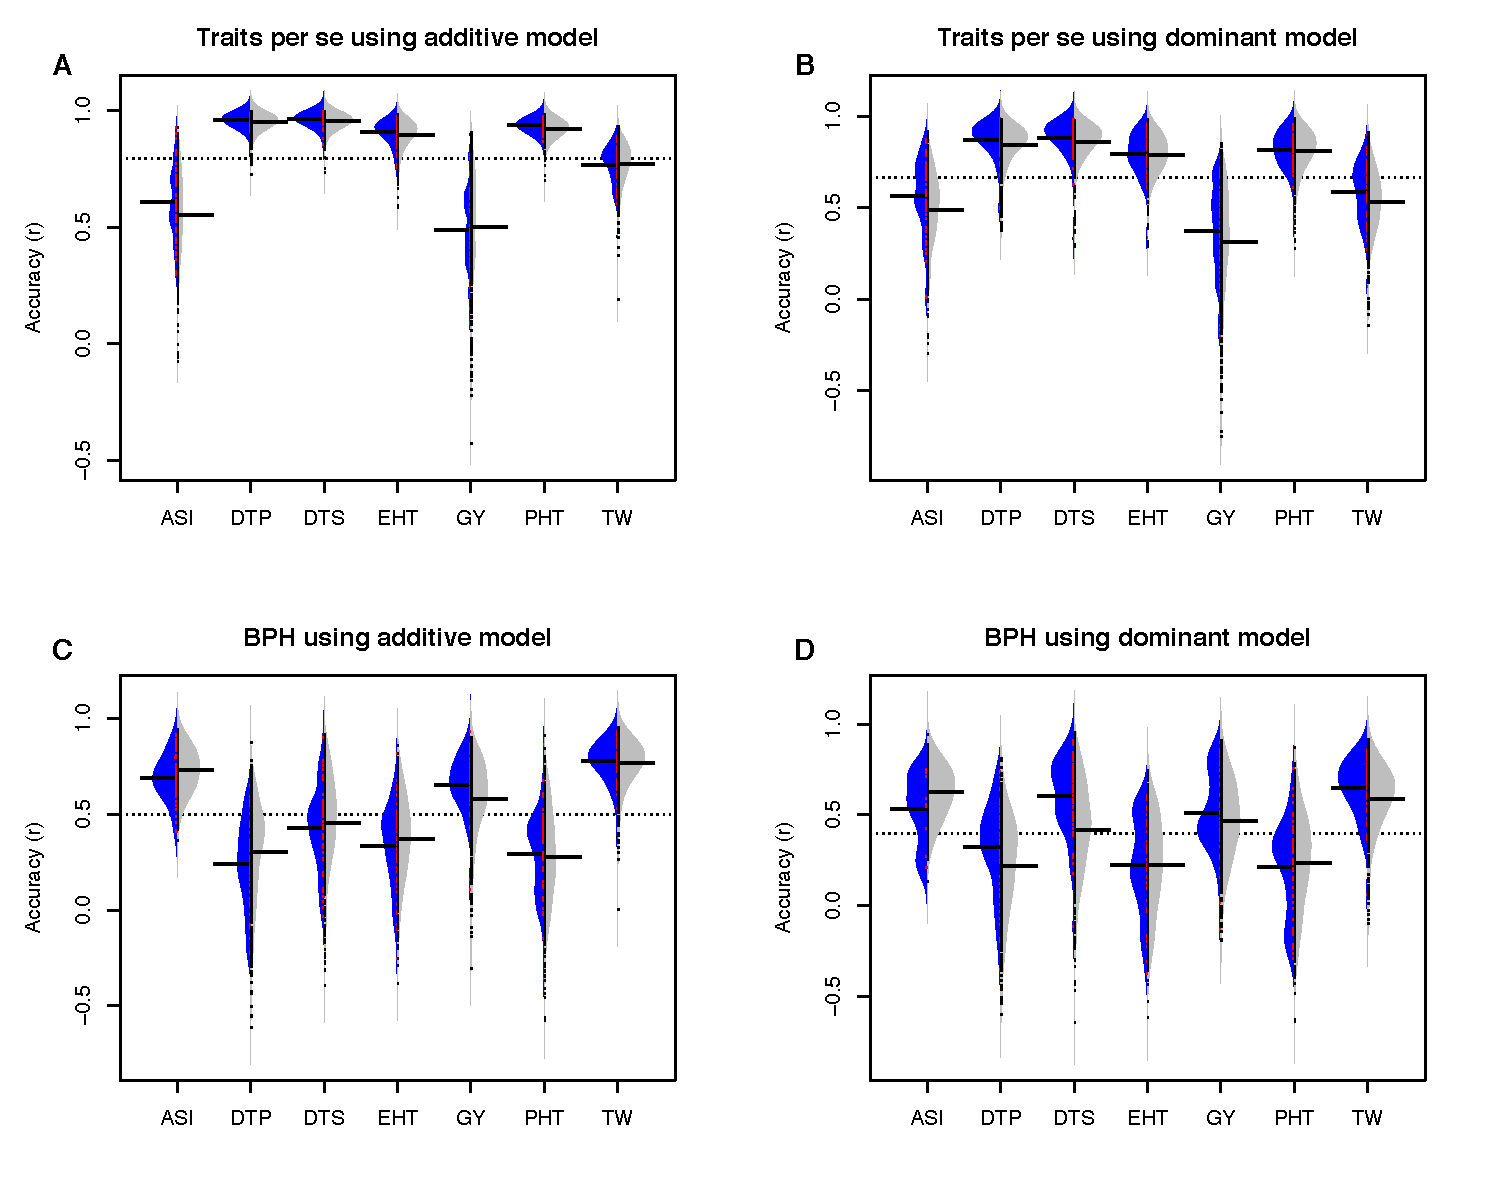
\includegraphics[width=\linewidth]{Figure_gerpall.pdf}
\caption{Beanplots of cross-validation accuracies using SNPs with positive GERP score. Cross-validation experiments were conducted using selected SNPs and circular shuffled data from the same set of SNPs for traits \emph{per se} (\textbf{A, B}), \DIFdelbeginFL \DIFdelFL{HPH }\DIFdelendFL \DIFaddbeginFL \DIFaddFL{BPH }\DIFaddendFL (\textbf{C, D}) and \DIFdelbeginFL \DIFdelFL{pHPH }\DIFdelendFL \DIFaddbeginFL \DIFaddFL{pBPH }\DIFaddendFL (\textbf{E, F}) under additive (\textbf{A, C, E}) and dominant (\textbf{B, D, F}) models. Accuraries from the real data were plotted on the left side of the bean (blue) and permutation results plotted on the right (grey). Horizotal bars on beans indicate mean accuracies. The grey dashed lines indicate the overall average accuracies. Stars indicate significantly improved cross-validation accuracies with FDR < 0.05.}
\label{fig:gerpall}
\end{figure}


\subsection*{Posterior phenotypic variance explained and model comparisons}

To learn why the prediction performace varied among traits \emph{per se} and heterosis transformations, we obtained the posterior variance explained by our models using the complete set of data. As \DIFdelbegin \DIFdel{expected, for most of the phenotypes, higher posterior variance could be explained for }\DIFdelend \DIFaddbegin \DIFadd{shown in Figure \ref{fig:h2}, additive models explained more phenotypic variance for }\DIFaddend traits \DIFdelbegin \emph{\DIFdel{per se}} \DIFdel{than BPHand pBPH using }\DIFdelend \DIFaddbegin \emph{\DIFadd{per se}} \DIFadd{of DTP, DTS, EHT and PHT; but explained less phenotypic variance for heterosis transformations (BPH) of ASI, GY and TW. On the contrary, lager proportions of the phenotypic variance could be explained by the dominant models for heterosis transformations (BPH) of ASI, GY and TW. For the GY in particular, 50\% of the heterosis could be explained by dominant model.   
}

\DIFadd{Heterosis transformations were largely determined by the accuracies of the parental phenotypes. To take the uncertainty of the parental phenotypes into consideration, we estimated the combining abilities from the hybrid population itself to investigate which modes of inheritance perform better than the null models. We extracted the breeding values estimated with both additive and dominant models using the }\DIFaddend genome-wide \DIFdelbegin \DIFdel{IBD blocks incorporated with GERP scores. }\DIFdelend \DIFaddbegin \DIFadd{IBD blocks incorporated with the GERP scores. Consistent with above analysis, IBD blocks coded with dominant mode of inheritance significantly (equation \ref{eq:refname1} vs. equation \ref{eq:refname2}, ANOVA }\emph{\DIFadd{P}} \DIFadd{value < 0.05 ) improved model fitting for ASI and GY. We also compared model \ref{eq:refname3} and model \ref{eq:refname4}, ANOVA results indicated that \ref{eq:refname4} performed almost as good as \ref{eq:refname3}, indicating that specific combining ability captured most of the parental interactions and the current method could not detect higher order of interactions. 
}\DIFaddend 

\DIFdelbegin \DIFdel{were observed using all the conserved SNPs as compared to the genic SNPs (Table SN) . For most of the traits }\emph{\DIFdel{per se}}\DIFdel{, phenotypic variance could be largely explained (posterior variance explained by markers range from 0.9 to 0.8 with additive model; with dominant model). But, it became difficult to explain heterosis transformations. Figure \ref{fig:h2}
}
\DIFdel{GCA and SCA
}
\DIFdel{and the breeding values. 
Breeding values from the BeyesC models were extracted. The below four models were compared. 
}
\DIFdelend \begin{equation}
Y_{ij} = \mu + GCA_{i} + GCA_{j} + \varepsilon
\label{eq:refname1}
\end{equation}
\begin{equation}
Y_{ij} = \mu + GCA_{i} + GCA_{j} +  G_{ij} + \varepsilon
\label{eq:refname2}
\end{equation}
\begin{equation}
Y_{ij} = \mu + GCA_{i} + GCA_{j} + SCA_{ij} + \varepsilon
\label{eq:refname3}
\end{equation}
\begin{equation}
Y_{ij} = \mu + GCA_{i} + GCA_{j} + SCA_{ij} + G_{ij} + \varepsilon
\label{eq:refname4}
\end{equation}
where 
$Y_{ij}$ is the BLUE value of the hybrid crossed between the $i^{th}$ inbred and $j^{th}$ inbred; 
$\mu$, the overall mean; 
$GCA_{i}$, the general combining ability of the $i^{th}$ inbred;
$GCA_{j}$, the general combining ability of the $j^{th}$ inbred;
$SCA_{ij}$, the specific combining ability of between the $i^{th}$ and $j^{th}$ inbreds;
$\varepsilon$, the model residuals.

\DIFdelbegin \DIFdel{1. It capture high order of interactions.  
}
\DIFdel{2. Explainary variables came from the centeromic regions.
}
\DIFdel{TO DO:
0. preparing all the traits (per se, HPH, MPH, pHPH and pMPH)
1. comparing same no. of random SNPs vs. GERP SNPs without considering their SCORE.
2. comparing MAF in different caterigories
3. training all the data and get the idea of significant ones.
}
\DIFdelend \begin{figure}[htbp]
\centering
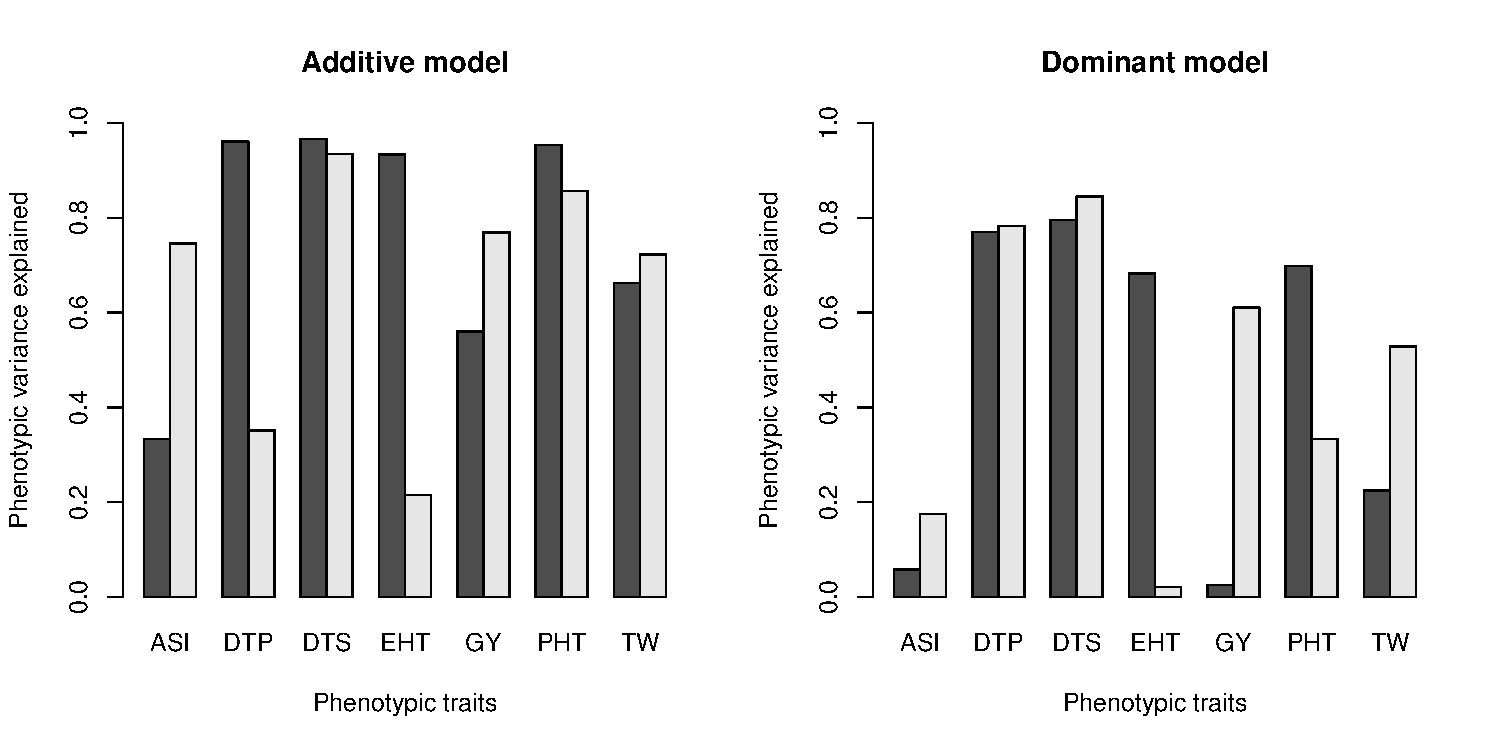
\includegraphics[width=\linewidth]{Figure_h2.pdf}
\caption{Barplots of the phenotypic variance explained by IBD blocks incorporated with GERP scores.}
\label{fig:h2}
\end{figure}


\section*{Discussion}

\begin{itemize}
  \item how do results match with heritability and heterosis?
  \item do we support deleterious model of Mezmouk et al.?
\end{itemize}


\DIFdelbegin \DIFdel{Schmitt: How to explain the prediction difference?  
- First, broad sense heritability of the traits are different. Second, from the simulation we learned that different traits may controlled by different proportion of additive, dominant and even recessive gene actions. Our naive model only built the pure additive and pure dominant effects in. For the more complicated cases, the models may not work very well.
}
\DIFdelend In this study, more than 500,000 deleterious SNPs were identified in elite maize lines including in \DIFdelbegin \DIFdel{noncoding }\DIFdelend \DIFaddbegin \DIFadd{non-coding }\DIFaddend regions of the genome. Majority of them were maintained in a low frequency, which consistent with the previous observation \DIFdelbegin \DIFdel{and indicate }\DIFdelend \DIFaddbegin \DIFadd{\mbox{\citep{rodgers2015recombination}
}and indicated }\DIFaddend the deleteriousness of the variants in the conserved sites. \DIFdelbegin \DIFdel{A }\DIFdelend \DIFaddbegin \DIFadd{To estimate the joint effects of the potentical deleterious alleles for the phenotype, a }\DIFaddend genomic selection pipeline was developed, which utilized evolutionary conservation information in the \DIFdelbegin \DIFdel{model. Cross-validation }\DIFdelend \DIFaddbegin \DIFadd{IBD blocks as explainatroy variables. After model training, cross-validation }\DIFaddend results suggested prediction accuracies for some traits \DIFaddbegin \emph{\DIFadd{per se}} \DIFadd{and heterosis transformations }\DIFaddend could be significantly improved by incorporating GERP scores. 

\DIFaddbegin \DIFadd{Paritcally, with dominant model, up to 20\% of the phenotypic variance could be explained for the heterosis traits. Theoritically, BPH transformation subtracts the joint effects of the additive and dominant alleles in the best parents as residule, the substantiall variance of these redidules explained by the additive or dominant models in our studies indicated that genetic components controlling for heterosis might in linked state. Note that the current model simply assume the traits were simply determined by complete additive or complete dominant. In the real case, the phenotype most likely be controlled by some degree of mixture of additive and dominant complenents. 
}

\DIFadd{Schmitt: How to explain the prediction difference?  
The variation of the prediction accuacies were relative large in this study. First of all, broad sense heritability of the traits are different. Second, from the simulation we learned that different traits may controlled by different proportion of additive, dominant and even recessive gene actions. Our naive model only built the pure additive and pure dominant effects in. For the more complicated cases, the models may not work very well.
}\DIFaddend 
\clearpage
\bibliography{Diallel}


\pagebreak
\beginsupplement
\section*{Supporting Information}

\DIFaddbegin \onecolumn
\DIFaddend \begin{center}\vspace{1cm}
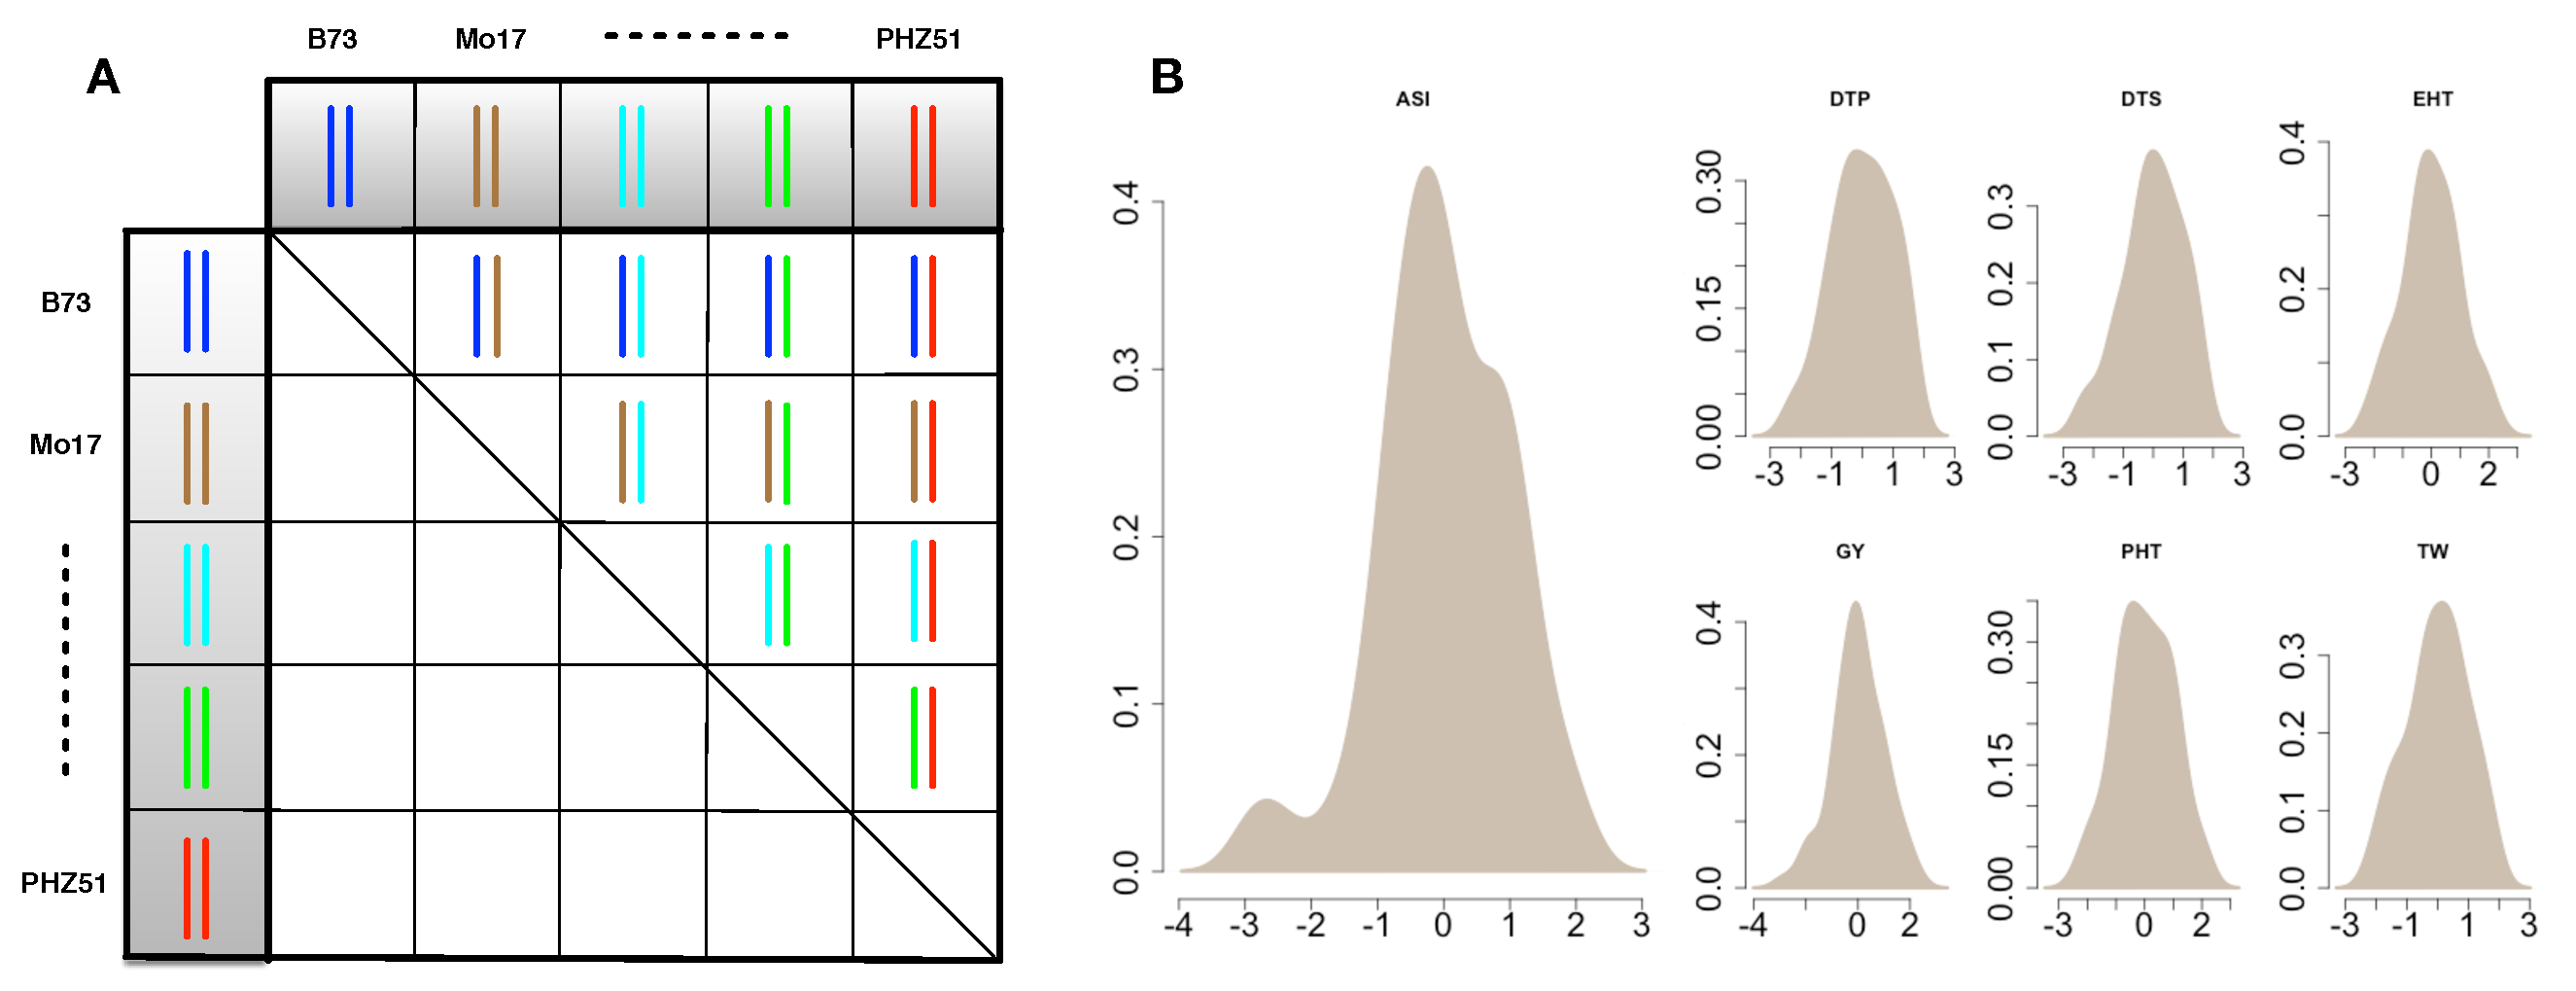
\includegraphics[width=0.8\linewidth]{SFig_pvp.pdf}
\captionof{figure}
{\color{black} \textbf{Diallel experimental design and distribution of phenotypic data.}
\textbf{(A)} Twelve maize inbred lines were selected and crossed in a \DIFdelbegin \DIFdel{half diallel. Ten of these (LH1, LH123HT, LH82, PH207, 4676A, PHG39, PHG47, PHG84, PHJ40, PHZ51) are proprietary inbreds that have expired from Plant Variety Protection (PVP) and represent the lineage of key heterotic germplasm pools used in present-day commercial corn hybrids.
Two of them are important public inbreds, B73 and Mo17. }\DIFdelend \DIFaddbegin \DIFadd{partial diallel. }\jri{do we need to modify this diagram now that we now reciprocal crosses were pooled?} \DIFaddend \textbf{(B)} \DIFdelbegin \DIFdel{Phenotypic data were collected for anthesis-silking interval (ASI, in days), days to 50\% pollen shed (DTP), days to 50\% silking (DTS), ear height (EHT, in cm), grain yield adjusted to 15.5\% moisture (GY, in bu/A), plant height (PHT, in cm), and test weight (TW, in pounds). Analyses were carried out on the traits per se as well as percent high parent heterosis (pHPH).
}\DIFdelend \DIFaddbegin \DIFadd{Density plots of the phenotypic distributions.
}\DIFaddend }
\label{fig:pvp-pheno}
\end{center}\vspace{1cm}

\begin{figure}[htbp]
\centering
\DIFaddbeginFL 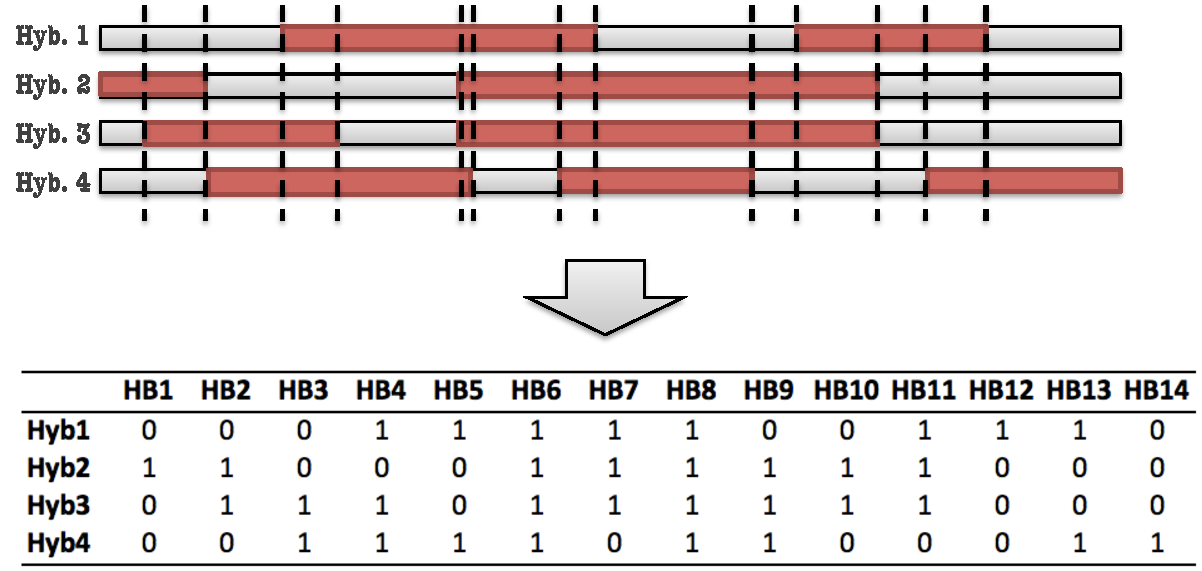
\includegraphics[width=\linewidth]{SFig_define_IBD.pdf}
\caption{\DIFaddFL{Haplotype block identification using an IBD approach. In the upper panel, regions in red are IBD blocks identified by pairwise comparison of the two parental lines of a hybrid. The vertical dashed lines define haplotype blocks. In the lower panel, hybrid genotypes at each block are coded as heterozygotes (0) or homozygotes (1).}}
\label{fig:defineibd}
\end{figure}



\begin{figure}[htbp]
\centering
\DIFaddendFL \includegraphics[width=\linewidth]{SFig_pBPH.pdf}
\caption{Boxplot of  \DIFdelbeginFL \DIFdelFL{the }\DIFdelendFL percent \DIFdelbeginFL \DIFdelFL{better parental }\DIFdelendFL \DIFaddbeginFL \DIFaddFL{best parent }\DIFaddendFL heterosis (pBPH). In the plot, ASI was calculated using pBPHmin and the other six traits were calculated using pBPHmax.}
\label{fig:pBPH}
\end{figure}

\begin{figure}[htbp]
\centering
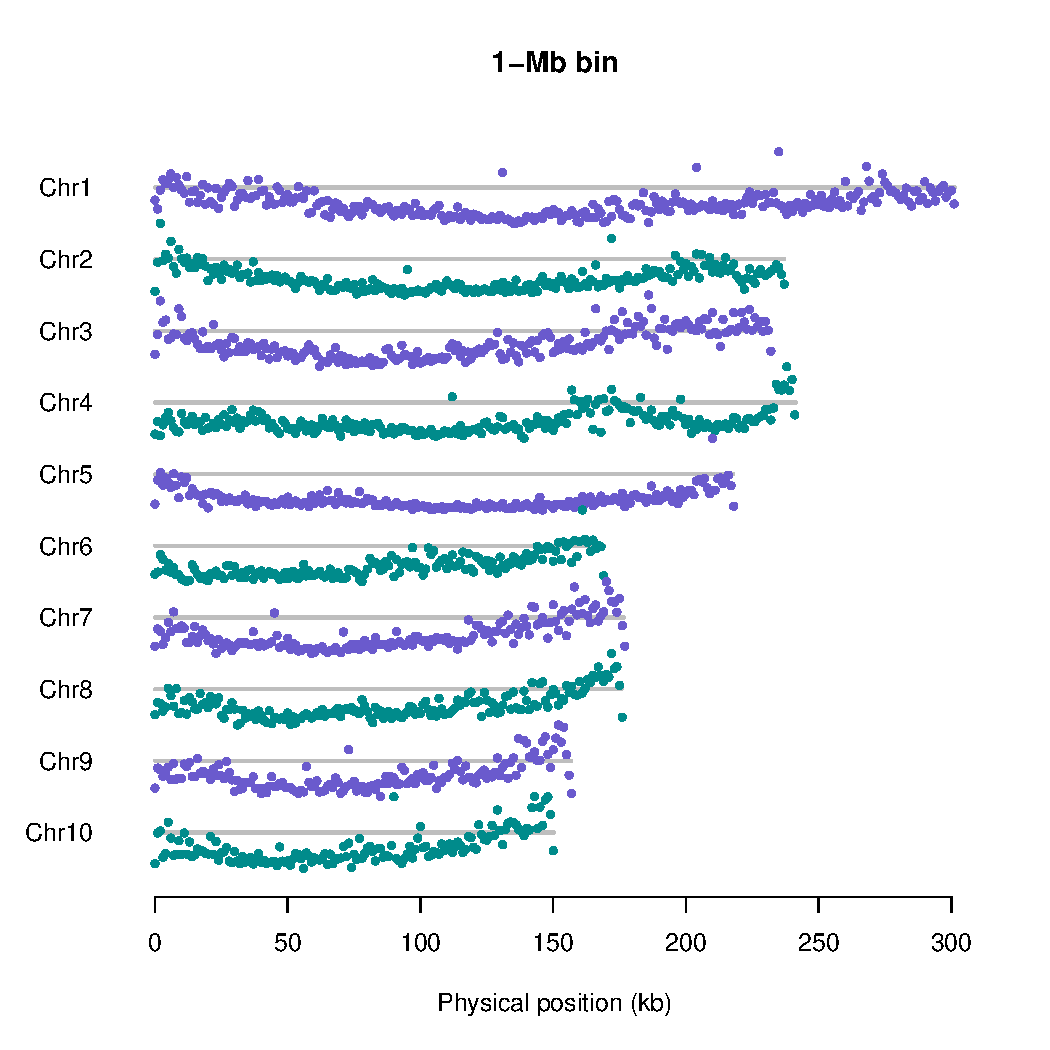
\includegraphics[width=\linewidth]{SFig_gerp_dis1m.pdf}
\caption{GERP score distribution across the genome. \DIFdelbeginFL \DIFdelFL{On the y-axis }\DIFdelendFL \DIFaddbeginFL \DIFaddFL{Shown }\DIFaddendFL are \DIFdelbeginFL \DIFdelFL{the }\DIFdelendFL mean GERP scores in a 1-Mb bin region.}
\label{fig:dis1m}
\end{figure}

\DIFdelbegin \DIFdelend \DIFaddbegin \begin{figure}[h]
\DIFaddendFL 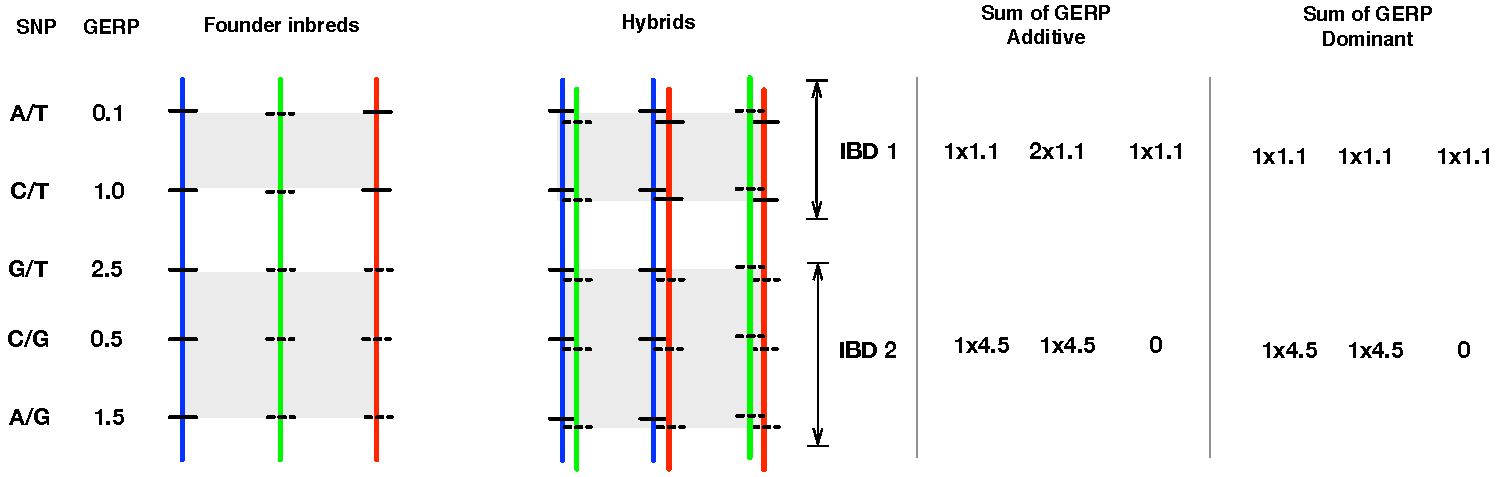
\includegraphics[width=0.9\textwidth]{SFig_gerpIBD.pdf}
\caption{
\textbf{Incoporation of conservation information into IBD blocks.}
Regions of the genome that are identical by descent (IBD) among the 12 inbreds were identified using Beagle \citep{Browning2009}.  The GERP scores of SNPs in an IBD block were summed under both additive and dominant models. \DIFdelbeginFL \DIFdelFL{Under the additive model, 2 x }\DIFdelendFL \DIFaddbeginFL \DIFaddFL{For a particular SNP with }\DIFaddendFL GERP score \DIFdelbeginFL \DIFdelFL{was assigned to genotypes homozygous for }\DIFdelendFL \DIFaddbeginFL \DIFaddFL{$g$, }\DIFaddendFL the \DIFaddbeginFL \DIFaddFL{homozygous }\DIFaddendFL non-reference \DIFdelbeginFL \DIFdelFL{allele, 1 x GERP score }\DIFdelendFL \DIFaddbeginFL \DIFaddFL{genotype }\DIFaddendFL was assigned \DIFdelbeginFL \DIFdelFL{to heterozygotes}\DIFdelendFL \DIFaddbeginFL \DIFaddFL{a value of $2g$}\DIFaddendFL , \DIFdelbeginFL \DIFdelFL{and 0 was }\DIFdelendFL \DIFaddbeginFL \DIFaddFL{the heterozygote }\DIFaddendFL assigned \DIFdelbeginFL \DIFdelFL{to }\DIFdelendFL \DIFaddbeginFL \DIFaddFL{a value of $g$, and }\DIFaddendFL the \DIFdelbeginFL \DIFdelFL{homozygous }\DIFdelendFL reference \DIFdelbeginFL \DIFdelFL{genotype. }\DIFdelendFL \DIFaddbeginFL \DIFaddFL{homozygote a value of 0.  }\DIFaddendFL Under the dominant model, \DIFdelbeginFL \DIFdelFL{1 x GERP score was assigned to }\DIFdelendFL both \DIFdelbeginFL \DIFdelFL{genotypes with a nonreference allle }\DIFdelendFL \DIFaddbeginFL \DIFaddFL{the heterozygote }\DIFaddendFL and \DIFdelbeginFL \DIFdelFL{0 to }\DIFdelendFL the \DIFdelbeginFL \DIFdelFL{homozygous }\DIFdelendFL \DIFaddbeginFL \DIFaddFL{non-reference homozygote were assigned a value of $g$, with the }\DIFaddendFL reference \DIFdelbeginFL \DIFdelFL{genotype.}\DIFdelendFL \DIFaddbeginFL \DIFaddFL{homozygote again assigned a value of 0.}\DIFaddendFL }
\label{fig:gerpibd}
\end{figure}

\begin{figure}[htbp]
\centering
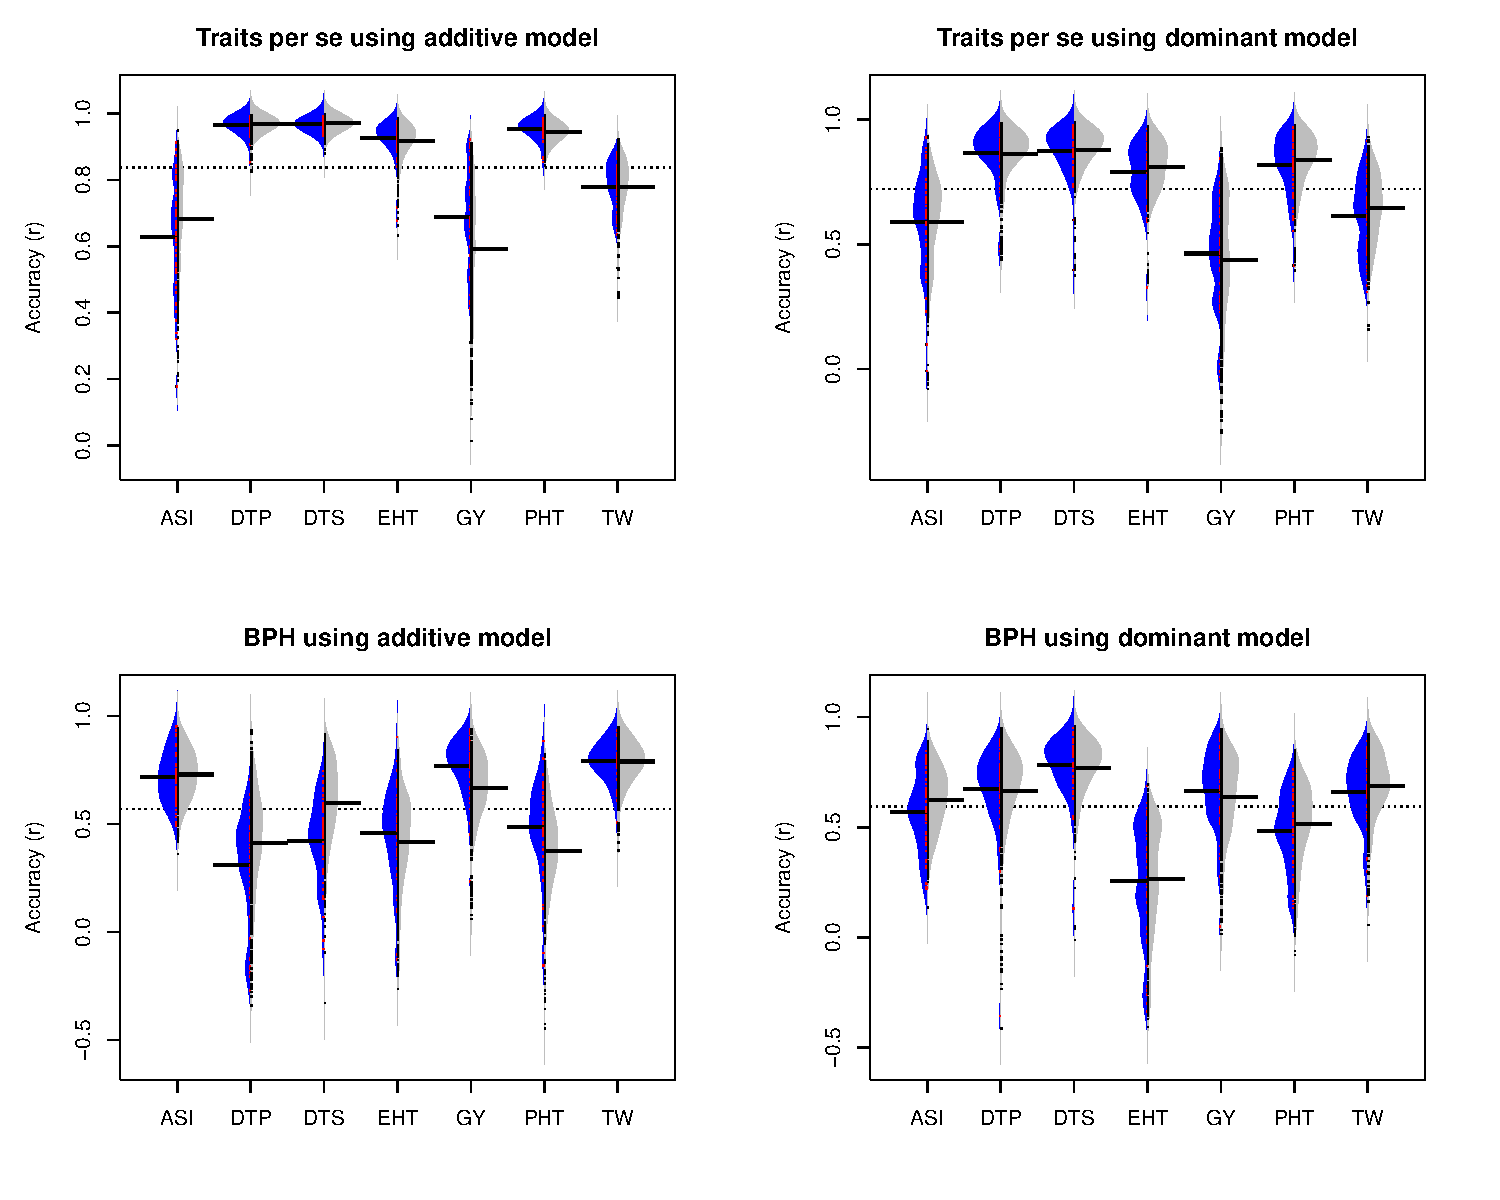
\includegraphics[width=\linewidth]{SFig_genicsnp.pdf}
\caption{\DIFdelbeginFL \DIFdelFL{Beanplots of cross-validation }\DIFdelendFL \DIFaddbeginFL \DIFaddFL{Cross-validation }\DIFaddendFL accuracies using genic SNPs. Cross-validation experiments were conducted using genic SNPs and \DIFdelbeginFL \DIFdelFL{circular shuffled }\DIFdelendFL \DIFaddbeginFL \DIFaddFL{compared to circular-shuffled }\DIFaddendFL data \DIFdelbeginFL \DIFdelFL{from the same set of the genic SNPs }\DIFdelendFL for traits \emph{per se} (\textbf{A, B}) and \DIFdelbeginFL \DIFdelFL{pHPH }\DIFdelendFL \DIFaddbeginFL \DIFaddFL{pBPH }\DIFaddendFL (\textbf{C, D}) under additive (\textbf{A, C}) and dominant (\textbf{B, D}) models. \DIFdelbeginFL \DIFdelFL{Accuaries }\DIFdelendFL \DIFaddbeginFL \DIFaddFL{Distirbutions show accuracty of prediction }\DIFaddendFL from \DIFdelbeginFL \DIFdelFL{the }\DIFdelendFL real data \DIFdelbeginFL \DIFdelFL{were plotted on the left side of the bean }\DIFdelendFL (blue) and \DIFdelbeginFL \DIFdelFL{permutation results plotted on the right }\DIFdelendFL \DIFaddbeginFL \DIFaddFL{permutations }\DIFaddendFL (grey)\DIFdelbeginFL \DIFdelFL{. Horizotal }\DIFdelendFL \DIFaddbeginFL \DIFaddFL{, with horizontal }\DIFaddendFL bars \DIFdelbeginFL \DIFdelFL{on beans }\DIFdelendFL \DIFaddbeginFL \DIFaddFL{to }\DIFaddendFL indicate mean \DIFdelbeginFL \DIFdelFL{accuracies. The grey dashed line indicates the overall average }\DIFdelendFL accuracy.  Stars indicate significantly \DIFdelbeginFL \DIFdelFL{improved }\DIFdelendFL \DIFaddbeginFL \DIFaddFL{higher }\DIFaddendFL cross-validation \DIFdelbeginFL \DIFdelFL{accuracies}\DIFdelendFL \DIFaddbeginFL \DIFaddFL{accuracy for the real data.  The average accuracy across all traits is shown with the grey dotted line}\DIFaddendFL . }
\label{fig:genicsnp}
\end{figure}

\end{document}